\documentclass[12pt,a4paper]{article}

% ── Packages ──────────────────────────────────────────────
\usepackage[a4paper, margin=2.5cm]{geometry}
\usepackage{fontenc}
\usepackage{inputenc}
\usepackage{lmodern}
\usepackage{microtype}
\usepackage{xcolor}
\usepackage{graphicx}
\usepackage{booktabs}
\usepackage{longtable}
\usepackage{array}
\usepackage{tabularx}
\usepackage{enumitem}
\usepackage{titlesec}
\usepackage{titletoc}
\usepackage{fancyhdr}
\usepackage{hyperref}
\usepackage{listings}
\usepackage{tcolorbox}
\usepackage{mdframed}
\usepackage{amssymb}
\usepackage{pifont}
\usepackage{parskip}
\usepackage{setspace}
\usepackage{afterpage}
\usepackage{tikz}

% ── Colors ────────────────────────────────────────────────
\definecolor{primary}{RGB}{37, 99, 235}
\definecolor{darkbg}{RGB}{15, 23, 42}
\definecolor{lightgray}{RGB}{248, 250, 252}
\definecolor{bordergray}{RGB}{226, 232, 240}
\definecolor{textgray}{RGB}{100, 116, 139}
\definecolor{successgreen}{RGB}{22, 163, 74}
\definecolor{warningyellow}{RGB}{217, 119, 6}
\definecolor{dangerred}{RGB}{220, 38, 38}
\definecolor{codebg}{RGB}{241, 245, 249}
\definecolor{codecomment}{RGB}{100, 116, 139}

% ── Hyperref Setup ────────────────────────────────────────
\hypersetup{
    colorlinks=true,
    linkcolor=primary,
    urlcolor=primary,
    citecolor=primary,
    pdftitle={Zetra Electronics Deployment Handover Document},
    pdfauthor={The Ark Tech},
    pdfsubject={Project Handover},
    bookmarks=true,
    bookmarksnumbered=true
}

% ── Section Styling ───────────────────────────────────────
\titleformat{\section}
  {\Large\bfseries\color{darkbg}}
  {\thesection.}{0.8em}{}
  [\vspace{0.1em}\color{primary}\rule{\linewidth}{1.5pt}]

\titleformat{\subsection}
  {\large\bfseries\color{darkbg}}
  {\thesubsection}{0.8em}{}

\titleformat{\subsubsection}
  {\normalsize\bfseries\color{primary}}
  {}{0em}{}

\titlespacing*{\section}{0pt}{2em}{0.8em}
\titlespacing*{\subsection}{0pt}{1.5em}{0.5em}
\titlespacing*{\subsubsection}{0pt}{1em}{0.3em}

% ── Header & Footer ───────────────────────────────────────
\pagestyle{fancy}
\fancyhf{}
\fancyhead[L]{\small\color{textgray}Zetra Electronics — Deployment Handover Document}
\fancyhead[R]{\small\color{textgray}The Ark Tech}
\fancyfoot[C]{\small\color{textgray}\thepage}
\renewcommand{\headrulewidth}{0.4pt}
\renewcommand{\footrulewidth}{0pt}
\renewcommand{\headrule}{\color{bordergray}\hrule width\headwidth height\headrulewidth}

% ── Code Listing Style ────────────────────────────────────
\lstset{
    backgroundcolor=\color{codebg},
    basicstyle=\small\ttfamily\color{darkbg},
    commentstyle=\color{codecomment},
    keywordstyle=\color{primary}\bfseries,
    stringstyle=\color{successgreen},
    breaklines=true,
    breakatwhitespace=true,
    frame=single,
    rulecolor=\color{bordergray},
    framesep=8pt,
    xleftmargin=12pt,
    xrightmargin=12pt,
    numbers=none,
    showstringspaces=false,
    tabsize=2,
    aboveskip=8pt,
    belowskip=8pt
}

% ── Custom Boxes ──────────────────────────────────────────
\tcbuselibrary{skins, breakable}

\newtcolorbox{infobox}{
    enhanced, breakable,
    colback=blue!5!white,
    colframe=primary,
    boxrule=0.8pt,
    arc=4pt,
    left=10pt, right=10pt, top=8pt, bottom=8pt,
    fonttitle=\bfseries\color{primary}
}

\newtcolorbox{warningbox}{
    enhanced, breakable,
    colback=yellow!10!white,
    colframe=warningyellow,
    boxrule=0.8pt,
    arc=4pt,
    left=10pt, right=10pt, top=8pt, bottom=8pt
}

\newtcolorbox{archbox}{
    enhanced, breakable,
    colback=darkbg,
    colframe=darkbg,
    boxrule=0pt,
    arc=6pt,
    left=12pt, right=12pt, top=10pt, bottom=10pt
}

% ── Checkmark & Cross ─────────────────────────────────────
\newcommand{\cmark}{\textcolor{successgreen}{\ding{51}}}
\newcommand{\xmark}{\textcolor{dangerred}{\ding{55}}}

% ── Table Column Types ────────────────────────────────────
\newcolumntype{L}[1]{>{\raggedright\arraybackslash}p{#1}}
\newcolumntype{C}[1]{>{\centering\arraybackslash}p{#1}}

% ── Spacing ───────────────────────────────────────────────
\setlength{\parskip}{6pt}
\setlength{\parindent}{0pt}

% ════════════════════════════════════════════════════════════
\begin{document}
% ════════════════════════════════════════════════════════════

% ── Cover Page ────────────────────────────────────────────
\begin{titlepage}
\pagecolor{darkbg}
\afterpage{\nopagecolor}
\centering
\vspace*{3cm}

{\color{white}\fontsize{11}{14}\selectfont\texttt{DEPLOYMENT HANDOVER DOCUMENT}}\\[1.2cm]

{\color{white}\fontsize{36}{44}\selectfont\bfseries Zetra Electronics}\\[0.4cm]

{\color{primary}\fontsize{16}{20}\selectfont\itshape E-Commerce Platform}\\[2.5cm]


\begin{tikzpicture}
  \draw[color=primary, line width=1.5pt] (0,0) -- (12,0);
\end{tikzpicture}

\vspace{2cm}

\begin{tabular}{@{}L{5cm} L{7cm}@{}}
{\color{textgray}\small Prepared by} & {\color{white}\small The Ark Tech} \\[0.4cm]
{\color{textgray}\small Website} & {\color{primary}\small\texttt{https://zetraelectronics.com}} \\[0.4cm]
{\color{textgray}\small Date} & {\color{white}\small May 2026} \\[0.4cm]
{\color{textgray}\small Version} & {\color{white}\small 1.0} \\[0.4cm]
{\color{textgray}\small Document Type} & {\color{white}\small Confidential — Client Delivery} \\
\end{tabular}

\vfill

{\color{textgray}\small\itshape This document contains sensitive credentials and infrastructure details.\\
Handle with care and store securely.}

\end{titlepage}

% ── Table of Contents ─────────────────────────────────────
\newpage
\tableofcontents
\newpage

% ════════════════════════════════════════════════════════════
\section{Project Overview}
% ════════════════════════════════════════════════════════════

Zetra Electronics is a full-stack e-commerce platform built for selling electronic components online in India. It includes a customer-facing storefront and a complete admin panel for managing the business end-to-end.

\subsubsection{What the Platform Does}
\begin{itemize}[leftmargin=1.5em, itemsep=4pt]
  \item Customers can browse products, add to cart, and pay online via Razorpay (UPI, Cards, NetBanking)
  \item Admin can manage products, categories, orders, customers, and store settings
  \item Orders are tracked from placement to delivery with courier tracking support
  \item PDF invoices are automatically generated for every order
  \item GST, shipping fees, and tax calculations are handled automatically
  \item The platform is fully mobile responsive with dark mode support
  \item SEO optimized with sitemap, structured data, and meta tags
\end{itemize}

% ════════════════════════════════════════════════════════════
\section{System Architecture}
% ════════════════════════════════════════════════════════════

\begin{archbox}
\color{white}\ttfamily\small
\begin{verbatim}
  ┌──────────────────────────────────────────────────┐
  │         CUSTOMER / ADMIN BROWSER                 │
  └─────────────────┬────────────────────────────────┘
                    │  HTTPS
  ┌─────────────────▼────────────────────────────────┐
  │     NEXT.JS FRONTEND  (Port 3000)                │
  │     zetraelectronics.com  →  served via PM2      │
  └─────────────────┬────────────────────────────────┘
                    │  Internal API calls
  ┌─────────────────▼────────────────────────────────┐
  │     NESTJS BACKEND API  (Port 4000)              │
  │     zetraelectronics.com/api → served via PM2    │
  └─────────────────┬────────────────────────────────┘
                    │
  ┌─────────────────▼────────────────────────────────┐
  │     POSTGRESQL DATABASE  (Port 5432)             │
  │     Database: zetra_db                           │
  └──────────────────────────────────────────────────┘
\end{verbatim}
\end{archbox}

\vspace{0.5em}

\begin{tabular}{@{}L{4cm} L{9cm}@{}}
\toprule
\textbf{Component} & \textbf{Details} \\
\midrule
Hosting & Hostinger VPS — IP: \texttt{187.127.140.206} \\
Domain & \texttt{zetraelectronics.com} \\
Process Manager & PM2 (keeps both services running 24/7, auto-restarts on crash) \\
Database & PostgreSQL (\texttt{zetra\_db}) \\
\bottomrule
\end{tabular}

% ════════════════════════════════════════════════════════════
\section{Access Credentials}
% ════════════════════════════════════════════════════════════

\begin{warningbox}
\textbf{IMPORTANT:} Change all passwords immediately after receiving this document. Store credentials in a secure password manager (e.g., 1Password, Bitwarden).
\end{warningbox}

\subsection{Website Admin Panel}

\begin{tabular}{@{}L{4cm} L{9cm}@{}}
\toprule
\textbf{Field} & \textbf{Value} \\
\midrule
URL & \texttt{https://zetraelectronics.com/admin} \\
Email & \texttt{admin@zetraelectronics.com} \\
Password & \textit{(provided separately)} \\
Role & ADMIN (full access) \\
\bottomrule
\end{tabular}

\subsection{VPS Server Access (SSH)}

\begin{tabular}{@{}L{4cm} L{9cm}@{}}
\toprule
\textbf{Field} & \textbf{Value} \\
\midrule
Host & \texttt{187.127.140.206} \\
Username & \texttt{root} \\
Password & \textit{(provided separately)} \\
SSH Command & \texttt{ssh root@187.127.140.206} \\
\bottomrule
\end{tabular}

\subsection{GitHub Repository}

\begin{tabular}{@{}L{4cm} L{9cm}@{}}
\toprule
\textbf{Field} & \textbf{Value} \\
\midrule
URL & \texttt{https://github.com/sherwynjoel/Tech-uc-e-commerce} \\
Branch & \texttt{main} \\
\bottomrule
\end{tabular}

\subsection{Database (PostgreSQL)}

\begin{tabular}{@{}L{4cm} L{9cm}@{}}
\toprule
\textbf{Field} & \textbf{Value} \\
\midrule
Host & \texttt{localhost} (on VPS only) \\
Database & \texttt{zetra\_db} \\
User & \texttt{zetra} \\
Password & In \texttt{/home/zetra/Tech-uc-e-commerce/apps/api/.env} \\
\bottomrule
\end{tabular}

% ════════════════════════════════════════════════════════════
\section{Customer-Facing Website}
% ════════════════════════════════════════════════════════════

\subsection{All Public Pages}

\begin{longtable}{@{}L{3.5cm} L{4cm} L{6cm}@{}}
\toprule
\textbf{Page} & \textbf{URL} & \textbf{Description} \\
\midrule
\endfirsthead
\toprule
\textbf{Page} & \textbf{URL} & \textbf{Description} \\
\midrule
\endhead
Homepage & \texttt{/} & Hero section, featured products, category grid \\[4pt]
All Products & \texttt{/products} & Full catalog with filters and search \\[4pt]
Product Detail & \texttt{/products/\{id\}} & Images, specs, add to cart \\[4pt]
Shopping Cart & \texttt{/cart} & View and edit cart items \\[4pt]
Checkout & \texttt{/checkout} & Address, payment, order placement \\[4pt]
Order Success & \texttt{/checkout/success} & Confirmation after payment \\[4pt]
Track Orders & \texttt{/track-order} & Order history and live status \\[4pt]
Login & \texttt{/login} & Email/password and Google login \\[4pt]
Register & \texttt{/register} & New customer account creation \\[4pt]
Forgot Password & \texttt{/forgot-password} & Password reset request \\[4pt]
Contact & \texttt{/contact} & Contact form \\[4pt]
Help & \texttt{/help} & FAQ page \\[4pt]
Privacy Policy & \texttt{/privacy} & Privacy policy \\[4pt]
Terms of Service & \texttt{/terms} & Terms and conditions \\
\bottomrule
\end{longtable}

\subsection{Navigation Features}

\begin{itemize}[leftmargin=1.5em, itemsep=4pt]
  \item \textbf{Top bar (desktop):} Store phone, email, Track Order link, Help Center
  \item \textbf{All Categories dropdown:} Dynamically loaded from admin panel
  \item \textbf{Search bar:} Live search across all products by name
  \item \textbf{Cart icon:} Shows item count badge in real time
  \item \textbf{Login / My Account:} Authentication buttons
  \item \textbf{Mobile menu:} Full hamburger menu with all categories and account links
\end{itemize}

% ════════════════════════════════════════════════════════════
\section{Admin Panel — Complete Guide}
% ════════════════════════════════════════════════════════════

\subsection{Accessing the Admin Panel}

\begin{enumerate}[leftmargin=2em, itemsep=4pt]
  \item Go to: \textbf{\texttt{https://zetraelectronics.com/admin}}
  \item Log in with your admin email and password
  \item You will be automatically redirected to the dashboard
\end{enumerate}

\begin{infobox}
Only accounts with the \textbf{ADMIN} role can access \texttt{/admin}. Regular customer accounts will be redirected away automatically.
\end{infobox}

\subsection{Dashboard (\texttt{/admin})}

The dashboard shows a real-time overview of the business:

\begin{tabular}{@{}L{4.5cm} L{8.5cm}@{}}
\toprule
\textbf{Card} & \textbf{What it shows} \\
\midrule
Total Revenue & Sum of all completed order payments \\
Total Orders & Number of all orders placed \\
Active Products & Number of products currently in catalog \\
Total Users & Number of registered customer accounts \\
\bottomrule
\end{tabular}

\vspace{0.5em}
\textbf{Sales Chart:} A line graph showing revenue over recent days/weeks.

\textbf{Recent Orders:} A table of the latest orders with status, customer, and amount.

\subsection{Products (\texttt{/admin/products})}

Shows a table of all products with product image thumbnail, name, category, price, stock count, and Edit/Delete buttons. Click column headers (\textbf{Name}, \textbf{Price}, \textbf{Stock}) to sort ascending or descending.

\subsection{Orders (\texttt{/admin/orders})}

Full list of all customer orders. Each row shows Order ID, date/time (Indian timezone), customer name, phone, city/state, status badge, total amount, and tracking URL.

\vspace{0.5em}
\textbf{Order Status Colours:}

\begin{tabular}{@{}L{1cm} L{3cm} L{8cm}@{}}
\toprule
& \textbf{Status} & \textbf{Meaning} \\
\midrule
\textcolor{warningyellow}{\rule{0.8em}{0.8em}} & PENDING & Payment received, not yet shipped \\
\textcolor{primary}{\rule{0.8em}{0.8em}} & SHIPPED & Dispatched with courier \\
\textcolor{successgreen}{\rule{0.8em}{0.8em}} & DELIVERED & Customer received the order \\
\textcolor{dangerred}{\rule{0.8em}{0.8em}} & CANCELLED & Order was cancelled \\
\bottomrule
\end{tabular}

\vspace{0.5em}
\textbf{Actions on each order:}
\begin{enumerate}[leftmargin=2em, itemsep=3pt]
  \item \textbf{View} — Opens full order details page
  \item \textbf{Print} — Opens a printable address label for the courier
  \item \textbf{Invoice} — Downloads a PDF invoice
  \item \textbf{Fulfill} — Panel to update status and add tracking URL
\end{enumerate}

\subsection{Customers (\texttt{/admin/customers})}

Lists all registered users with customer name and email, account role (CUSTOMER / ADMIN), total number of orders placed, and account creation date.

\subsection{Inventory (\texttt{/admin/inventory})}

Two tabs:

\textbf{Products Tab:} Search products by name; filter by category, price, and stock. Stock levels below 10 units are highlighted in \textcolor{dangerred}{\textbf{red}} as a low-stock warning.

\textbf{Categories Tab:} Create new categories (name + optional description) and delete existing ones. Categories here appear in the storefront navigation and product filters.

\subsection{Settings (\texttt{/admin/settings})}

Configure your entire store from this page. See Section~\ref{sec:settings} for full details.

% ════════════════════════════════════════════════════════════
\section{How to Add \& Manage Products}
% ════════════════════════════════════════════════════════════

\subsection{Adding a New Product}

\begin{enumerate}[leftmargin=2em, itemsep=4pt]
  \item Go to \textbf{Admin $\rightarrow$ Products} (\texttt{/admin/products})
  \item Click \textbf{"Add Product"} button (top right)
  \item Fill in the product form (see table below)
  \item Click \textbf{Save} — product is immediately live on the storefront
\end{enumerate}

\begin{tabular}{@{}L{3.5cm} L{6cm} L{3.5cm}@{}}
\toprule
\textbf{Field} & \textbf{Description} & \textbf{Example} \\
\midrule
Name & Product title & Arduino Uno R3 \\[4pt]
Description & What the product is & Microcontroller based on ATmega328P \\[4pt]
Price (₹) & Selling price & 599 \\[4pt]
Shipping Cost (₹) & Per-item shipping (0 = free) & 50 \\[4pt]
Category & Select from your categories & Development Boards \\[4pt]
Stock & Units available & 100 \\[4pt]
Image & Upload product photo & JPG / PNG \\[4pt]
Datasheet & URL to PDF datasheet (optional) & https://... \\[4pt]
Specs & Technical specs as JSON & \texttt{\{"Voltage":"5V"\}} \\
\bottomrule
\end{tabular}

\subsection{Editing a Product}

Go to \textbf{Admin $\rightarrow$ Products}, click the \textbf{Edit} (pencil) icon on any product row, update fields, then click \textbf{Save}.

\subsection{Deleting a Product}

Go to \textbf{Admin $\rightarrow$ Products}, click the \textbf{Delete} (trash) icon, and confirm. Deleting a product removes it from the catalog but preserves it in past orders.

\subsection{Managing Categories}

\begin{enumerate}[leftmargin=2em, itemsep=4pt]
  \item Go to \textbf{Admin $\rightarrow$ Inventory $\rightarrow$ Categories tab}
  \item Enter a category name and optional description
  \item Click \textbf{Add Category}
\end{enumerate}

Categories automatically appear in the storefront navigation dropdown, product filter sidebar, and homepage category grid.

\subsection{Adding Technical Specifications}

Specs are stored as JSON. Use this format:

\begin{lstlisting}[language={}]
{
  "Operating Voltage": "5V",
  "Clock Speed": "16 MHz",
  "Flash Memory": "32 KB",
  "Digital I/O Pins": "14",
  "Analog Input Pins": "6"
}
\end{lstlisting}

These display as a formatted table on the product page under \textit{Technical Specifications}.

\subsection{Image Upload Guidelines}

\begin{itemize}[leftmargin=1.5em, itemsep=3pt]
  \item Supported formats: JPG, PNG, WebP
  \item Recommended size: \textbf{800×800px} (square)
  \item Images are stored on the server at \texttt{/uploads/}
  \item You can also paste an external image URL
\end{itemize}

% ════════════════════════════════════════════════════════════
\section{How to Manage Orders}
% ════════════════════════════════════════════════════════════

\subsection{Order Lifecycle}

\begin{center}
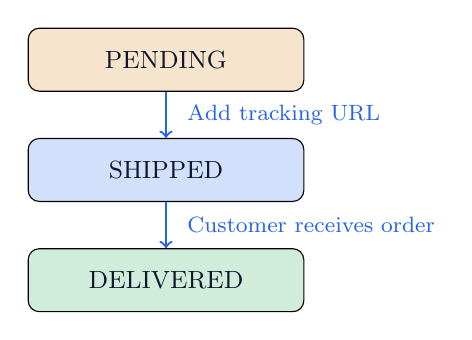
\begin{tikzpicture}[node distance=1.4cm, every node/.style={font=\small}]
  \node[draw, rounded corners, fill=warningyellow!20, text=darkbg, minimum width=3.5cm, minimum height=0.8cm] (p) {PENDING};
  \node[draw, rounded corners, fill=primary!20, text=darkbg, minimum width=3.5cm, minimum height=0.8cm, below of=p] (s) {SHIPPED};
  \node[draw, rounded corners, fill=successgreen!20, text=darkbg, minimum width=3.5cm, minimum height=0.8cm, below of=s] (d) {DELIVERED};
  \draw[->, thick, color=primary] (p) -- (s) node[midway, right, xshift=4pt] {\footnotesize Add tracking URL};
  \draw[->, thick, color=primary] (s) -- (d) node[midway, right, xshift=4pt] {\footnotesize Customer receives order};
\end{tikzpicture}
\end{center}

\subsection{Fulfilling an Order (Shipping)}

\begin{enumerate}[leftmargin=2em, itemsep=4pt]
  \item Go to \textbf{Admin $\rightarrow$ Orders}
  \item Find the order with \textbf{PENDING} status
  \item Click the \textbf{Fulfill} button on that order row
  \item In the panel that opens:
    \begin{itemize}
      \item Change \textbf{Status} to \textbf{SHIPPED}
      \item Paste the \textbf{Courier Tracking URL} (India Post, Delhivery, Bluedart, etc.)
    \end{itemize}
  \item Click \textbf{Update}
\end{enumerate}

The customer will then see the status change to ``Shipped'' on their Track Order page and can click the tracking link to follow their shipment.

\subsection{Printing an Address Label}

Click the \textbf{Print} button on any order row. A new window opens with a formatted shipping label. Print it from your browser (\texttt{Ctrl+P}).

The label includes:
\begin{itemize}[leftmargin=1.5em, itemsep=3pt]
  \item FROM: Zetra Electronics — zetraelectronics.com
  \item TO: Customer name, phone, full address, PIN code
  \item Order ID and date
\end{itemize}

\subsection{Downloading an Invoice}

Click the \textbf{Invoice} button on any order row. A PDF is generated with Order ID, customer billing address, itemized product list with quantities and prices, subtotal, shipping cost, GST amount, and final total.

\subsection{Cancelling an Order}

On the order detail page (\texttt{/admin/orders/\{id\}}), change the status to \textbf{CANCELLED}.

% ════════════════════════════════════════════════════════════
\section{Settings Configuration}
\label{sec:settings}
% ════════════════════════════════════════════════════════════

Go to \textbf{Admin $\rightarrow$ Settings} (\texttt{/admin/settings}). All settings auto-load when you open the page. After changes, click \textbf{Save Settings} (floating button, bottom right).

\subsection{Store Information}

\begin{tabular}{@{}L{5cm} L{8cm}@{}}
\toprule
\textbf{Setting} & \textbf{Description} \\
\midrule
Store Phone & Phone number shown in navbar and footer \\
Support Email & Email in navbar/footer; receives contact form messages \\
Store Address & Physical address shown in footer \\
\bottomrule
\end{tabular}

\subsection{Tax Configuration}

\begin{tabular}{@{}L{5cm} L{8cm}@{}}
\toprule
\textbf{Setting} & \textbf{Description} \\
\midrule
GST Percentage & Tax rate applied to all orders (default: 18\%) \\
\bottomrule
\end{tabular}

\subsection{Shipping Configuration}

\begin{tabular}{@{}L{5cm} L{8cm}@{}}
\toprule
\textbf{Setting} & \textbf{Description} \\
\midrule
Free Shipping Threshold & Minimum order value (₹) for free shipping \\
Standard Shipping Fee & Flat fee (₹) charged if threshold not met \\
\bottomrule
\end{tabular}

\textbf{Example:} If threshold = ₹500 and flat fee = ₹60:
\begin{itemize}[leftmargin=1.5em, itemsep=3pt]
  \item Order ₹499 $\rightarrow$ customer pays ₹60 shipping
  \item Order ₹500+ $\rightarrow$ free shipping
\end{itemize}

\subsection{Homepage Hero}

\begin{tabular}{@{}L{5cm} L{8cm}@{}}
\toprule
\textbf{Setting} & \textbf{Description} \\
\midrule
Hero Subtext & Tagline below the main heading on homepage \\
Hero Banner Image & Image shown on the right side of the hero section \\
\bottomrule
\end{tabular}

\subsection{Social Media Links}

\begin{tabular}{@{}L{5cm} L{8cm}@{}}
\toprule
\textbf{Setting} & \textbf{Description} \\
\midrule
Instagram URL & Full URL (e.g., \texttt{https://instagram.com/zetraelectronics}) \\
Twitter/X URL & Full URL \\
LinkedIn URL & Full URL \\
\bottomrule
\end{tabular}

These appear as icons in the website footer.

% ════════════════════════════════════════════════════════════
\section{Customer Workflow (End-to-End)}
% ════════════════════════════════════════════════════════════

\subsection{Step 1: Account Creation}
\begin{enumerate}[leftmargin=2em, itemsep=3pt]
  \item Customer visits \texttt{/register}
  \item Enters name, email, and password
  \item Account is created and logged in automatically
  \item \textit{(Optional)} Verify email via link sent to inbox
\end{enumerate}

\subsection{Step 2: Browsing Products}
\begin{itemize}[leftmargin=1.5em, itemsep=3pt]
  \item Browse by category via navbar dropdown or homepage grid
  \item Search by product name using the search bar
  \item Filter by category and price range on the \texttt{/products} page
  \item Click any product for full details, specs, and datasheet
\end{itemize}

\subsection{Step 3: Adding to Cart}
\begin{itemize}[leftmargin=1.5em, itemsep=3pt]
  \item Click \textbf{Add to Cart} on product card or detail page
  \item Cart icon in navbar shows live item count
  \item Visit \texttt{/cart} to review, update quantities, or remove items
\end{itemize}

\subsection{Step 4: Checkout}
\begin{enumerate}[leftmargin=2em, itemsep=3pt]
  \item Visit \texttt{/checkout}
  \item Fill in shipping address (First Name, Last Name, Phone, Street, PIN Code)
  \item PIN Code auto-fills City and State from Indian postal database
  \item Review Order Summary: items, subtotal, shipping fee, GST, final total
  \item Click \textbf{Place Order} — a confirmation modal appears
  \item Verify address and confirm
  \item Razorpay payment screen opens (UPI, Cards, NetBanking)
  \item Complete payment
  \item Redirected to \texttt{/checkout/success} with order confirmation
\end{enumerate}

\subsection{Step 5: Tracking the Order}
\begin{enumerate}[leftmargin=2em, itemsep=3pt]
  \item Visit \texttt{/track-order} (must be logged in)
  \item All orders listed with visual progress bar: Placed $\rightarrow$ Shipped $\rightarrow$ Delivered
  \item Click courier tracking link once admin marks as shipped
  \item Download PDF invoice for any order
\end{enumerate}

% ════════════════════════════════════════════════════════════
\section{Complete Feature List}
% ════════════════════════════════════════════════════════════

\subsection{Customer Features}

\begin{tabular}{@{}L{0.6cm} L{12cm}@{}}
\cmark & Browse products by category \\
\cmark & Search products by keyword \\
\cmark & Filter products by price range \\
\cmark & View product details, specifications, and datasheet \\
\cmark & Add / remove / update cart items \\
\cmark & Persistent cart (synced across devices when logged in) \\
\cmark & Guest cart preserved on login \\
\cmark & Checkout with Indian address form \\
\cmark & Auto PIN code lookup (city/state auto-fill) \\
\cmark & Razorpay payment (UPI, Cards, NetBanking) \\
\cmark & Order confirmation page \\
\cmark & Order tracking with visual progress bar \\
\cmark & Courier tracking link \\
\cmark & PDF invoice download \\
\cmark & Google OAuth login \\
\cmark & Email/password login with forgot password flow \\
\cmark & Order cancellation \\
\cmark & Dark mode support \\
\cmark & Fully mobile responsive \\
\cmark & Fast loading (Lighthouse optimized) \\
\end{tabular}

\subsection{Admin Features}

\begin{tabular}{@{}L{0.6cm} L{12cm}@{}}
\cmark & Dashboard analytics (revenue, orders, users, products) \\
\cmark & Sales chart visualization \\
\cmark & Add / edit / delete products \\
\cmark & Product image upload \\
\cmark & Technical specifications per product \\
\cmark & Datasheet PDF link per product \\
\cmark & Manage product categories \\
\cmark & View all customer orders \\
\cmark & Update order status (Pending $\rightarrow$ Shipped $\rightarrow$ Delivered) \\
\cmark & Add courier tracking URL to orders \\
\cmark & Print address labels \\
\cmark & Download order invoices \\
\cmark & View customer list \\
\cmark & Inventory management with low-stock alerts \\
\cmark & Store settings (phone, email, address, tax, shipping) \\
\cmark & Homepage hero image and text customization \\
\cmark & Social media links management \\
\end{tabular}

\subsection{Technical Features}

\begin{tabular}{@{}L{0.6cm} L{12cm}@{}}
\cmark & SEO optimized (meta tags, sitemap.xml, robots.txt) \\
\cmark & JSON-LD structured data (Google rich results) \\
\cmark & Security headers (CSP, HSTS, X-Frame-Options) \\
\cmark & JWT authentication \\
\cmark & Rate limiting (5 logins/min, 3 password resets/min) \\
\cmark & Account lockout after 10 failed login attempts \\
\cmark & Image optimization (WebP/AVIF via Next.js) \\
\cmark & Static asset caching (1 year) \\
\end{tabular}

% ════════════════════════════════════════════════════════════
\section{Technical Infrastructure}
% ════════════════════════════════════════════════════════════

\subsection{Technology Stack}

\begin{tabular}{@{}L{3cm} L{4.5cm} L{5cm}@{}}
\toprule
\textbf{Layer} & \textbf{Technology} & \textbf{Version} \\
\midrule
Frontend & Next.js (React) & 15 \\
Backend & NestJS & 11 \\
Database & PostgreSQL & — \\
ORM & Prisma & 5.22 \\
Styling & Tailwind CSS & 4 \\
Auth & JWT + Firebase Auth & — \\
Payments & Razorpay & — \\
Process Manager & PM2 & — \\
Hosting & Hostinger VPS & Ubuntu \\
\bottomrule
\end{tabular}

\subsection{Database Models}

\begin{tabular}{@{}L{3.5cm} L{9.5cm}@{}}
\toprule
\textbf{Table} & \textbf{Description} \\
\midrule
\texttt{User} & Customer and admin accounts with roles \\
\texttt{Product} & Product catalog with specs, images, and pricing \\
\texttt{Category} & Product categories \\
\texttt{CartItem} & Shopping cart items per user \\
\texttt{Order} & Customer orders with Razorpay payment info \\
\texttt{OrderItem} & Individual items within each order (price snapshot) \\
\texttt{SystemSetting} & Store configuration as key-value pairs \\
\bottomrule
\end{tabular}

\subsection{API Structure}

The backend API runs on port 4000 and is accessed internally by the frontend.

\begin{tabular}{@{}L{3cm} L{3cm} L{7cm}@{}}
\toprule
\textbf{Controller} & \textbf{Base Path} & \textbf{Key Endpoints} \\
\midrule
Auth & \texttt{/auth} & register, login, Google OAuth, password reset \\
Products & \texttt{/products} & CRUD + image upload \\
Orders & \texttt{/orders} & create, verify payment, fulfill, invoice PDF \\
Cart & \texttt{/cart} & add, remove, sync \\
Categories & \texttt{/categories} & create, list, delete \\
Settings & \texttt{/settings} & get all, update by key \\
Analytics & \texttt{/analytics} & dashboard stats, sales chart \\
Contact & \texttt{/contact} & send contact form email \\
\bottomrule
\end{tabular}

\subsection{Environment Variables}

Located at \texttt{/home/zetra/Tech-uc-e-commerce/apps/api/.env} on the VPS:

\begin{lstlisting}[language={}]
DATABASE_URL=postgresql://...
JWT_SECRET=...
RAZORPAY_KEY_ID=...
RAZORPAY_KEY_SECRET=...
FRONTEND_URL=https://zetraelectronics.com
SMTP_HOST=...
SMTP_USER=...
SMTP_PASS=...
\end{lstlisting}

% ════════════════════════════════════════════════════════════
\section*{Support \& Contact}
\addcontentsline{toc}{section}{Support \& Contact}
% ════════════════════════════════════════════════════════════

\vspace{0.5em}
\begin{tabular}{@{}L{4cm} L{9cm}@{}}
\textbf{Developer} & The Ark Tech \\[0.5em]
\textbf{Website}   & \texttt{https://thearktech.in} \\[0.5em]
\textbf{Email}     & \textit{(contact your developer)} \\
\end{tabular}

\vspace{1.5em}
\begin{center}

\begin{tikzpicture}
  \draw[color=bordergray, line width=1pt] (0,0) -- (13,0);
\end{tikzpicture}
\end{center}
\vspace{0.8em}

\begin{center}
\textit{\small This document was prepared as part of the project delivery for Zetra Electronics.\\
All credentials marked as ``provided separately'' will be delivered via a secure channel.}
\end{center}

\end{document}
